\documentclass[11pt]{article}
\usepackage[margin=1in]{geometry}
\usepackage{enumitem}
\usepackage{amsmath}
\usepackage[version=4]{mhchem}
\usepackage{tocloft}
\usepackage{graphicx}
\usepackage[colorlinks=true, linkcolor=blue, urlcolor=blue, citecolor=blue]{hyperref}

% Custom list setup for a tight, professional look
\setlist{nosep, leftmargin=*, topsep=2pt, partopsep=2pt}
\renewcommand{\labelitemi}{$\bullet$}

% Title formatting
\renewcommand{\maketitle}{
    \begin{center}
        {\LARGE \bfseries Bone} \\[0.5em]
        {\large KA Ansari} \\[1em]
    \end{center}
}

% Section formatting: Remove bold and add spacing
\renewcommand{\thesection}{\arabic{section}.}
\renewcommand{\thesubsection}{\thesection\arabic{subsection}.}


\usepackage[style=numeric, backend=biber]{biblatex} % verbose style is great for footnotes
\addbibresource{references.bib} % Load your .bib file (without the .bib extension)
% Adds "References" as the title for the bibliography
\renewcommand{\refname}{References}
\begin{document}

\maketitle

% Generate the Table of Contents
\tableofcontents
\newpage

\section{Definition}
Bone is a living, highly vascular, mineralized, constantly changing rigid specialized connective tissue that forms the framework of the body.\footnote{This definition as verbatim isn't mentioned in any textbook but almost all textbooks mention these properties of the bone. For a comprehensive overview, see \cite[p.~88]{gray2020}.}

Approximately 60-70\% of Bone dryweight is made up of inorganic mineral salts in the form of \textbf{microcrystalline hydroxyapatite} ($\ce{Ca10(PO4)6(OH)2}$). While Bone mineral also has important carbonate conent while also having Calcium Phosphate($\ce{Ca3(PO4)2}$)\cite[p.~90]{gray2020}.


\section{Properties}
\begin{itemize}
    \item Main constituent of the adult skeleton
    \item Contains calcified intercellular material—the bone matrix and bone cells
    \item Highly vascular and has nerve supply
    \item Has outer compact and inner spongy parts
    \item Acts as a reservoir of Calcium and phosphate
    \item Covered by periosteum, except the articular surface and sesamoid bones
\end{itemize}

\section{Function}
\begin{itemize}
    \item Forms rigid framework of body
    \item Carries weight
    \item Protection to the vital organs
    \item Bone marrow production
    \item Muscles, tendons, ligaments attachment (serve as levers for movement)
    \item Storehouse of calcium phosphate
    \item Contains bone marrow which manufactures blood cells
    \item Some bones afford protection to certain viscera
\end{itemize}

\section{Components}
\begin{itemize}
    \item \textbf{Cells (2\%)}
    \begin{itemize}
        \item Osteoprogenitor cells
        \item Osteoblast
        \item Osteocyte
        \item Osteoclast
    \end{itemize}
    \item \textbf{Intercellular matrix (98\%)}
\end{itemize}

\section{Periosteum}
\subsection{Definition}
Outer fibrovascular cellular covering of bone.

\subsection{Function}
\begin{itemize}
    \item Protect and cover
    \item Blood supply
    \item Attachment of muscles, tendon, ligaments
    \item Give shape and protect
    \item Increase girth
    \item Bone healing when fracture
    \item Helps in subperiosteal deposits of bone formation (increase the width)
    \item Protects the bone
    \item Gives nutrition to outer compact bone
\end{itemize}

\subsection{Layers}
\begin{itemize}
    \item \textbf{Outer fibrous layer}
    \item \textbf{Inner cellular vascular layer}
    \begin{itemize}
        \item Contains:
        \begin{itemize}
            \item Osteoprogenitor cell
            \item Osteoblast
        \end{itemize}
    \end{itemize}
\end{itemize}

\section{Classification}
\subsection{Morphological Classification}
Bones are classified according to their shape\footnote{Moore mentions only one classification and that is according to shape.\cite{moore2023}}.
\begin{itemize}
    \item Long Bone
    \item Short Bone
    \item Sesamoid Bone
    \item Flat Bone
    \item Irregular Bone
    \item Pneumatic Bone
    \item Accessory Bone
\end{itemize}

\subsubsection*{Long Bone}
\textbf{Types:}
\begin{itemize}
    \item \textbf{Typical Long Bone}
    \begin{itemize}
        \item \textbf{Example:} Radius, Femur
        \item \textbf{Features:}
        \begin{itemize}
            \item Long and roughly tubular shape
            \item Upper end, lower end \& intervening shaft
            \item Contains the medullary cavity
            \item Haversian system present
            \item \textbf{Development:} Cartilaginous ossification
            \item Primary ossification: Diaphysis and two epiphysis
            \item Lies vertically
            \item Carries weight
            \item Has three borders and surfaces
        \end{itemize}
    \end{itemize}
    
    \item \textbf{Modified Long Bone}
    \begin{itemize}
        \item \textbf{Example:} Clavicle
        \item \textbf{Features:}
        \begin{itemize}
            \item Horizontally placed
            \item Carries weight
            \item Haversian system absent
            \item Medullary cavity absent
            \item \textbf{Development:} Membranous ossification
        \end{itemize}
    \end{itemize}
    
    \item \textbf{Miniature Long Bone}
    \begin{itemize}
        \item \textbf{Example:} Metacarpal, Phalanges
        \item \textbf{Features:}
        \begin{itemize}
            \item One epiphyseal end, and one diaphysis
            \item Base is located at the epiphyseal end
        \end{itemize}
    \end{itemize}
\end{itemize}

\subsubsection*{Gross Structure of Long Bones}
\begin{itemize}
    \item Periosteum
    \item Compact bone
    \item Medullary cavity / Spongy bone
    \item Endosteum
\end{itemize}

\subsubsection*{Blood Supply}
As seen in \autoref{fig:blood_supply_of_bone} the bone is supplied by four arteries and on the inside is highly vascular
\begin{itemize}
    \item Nutrient Artery
    \item Periosteal Artery
    \item Epiphyseal Artery
    \item Metaphyseal Artery
\end{itemize}

\begin{figure}[htbp]
    \centering
    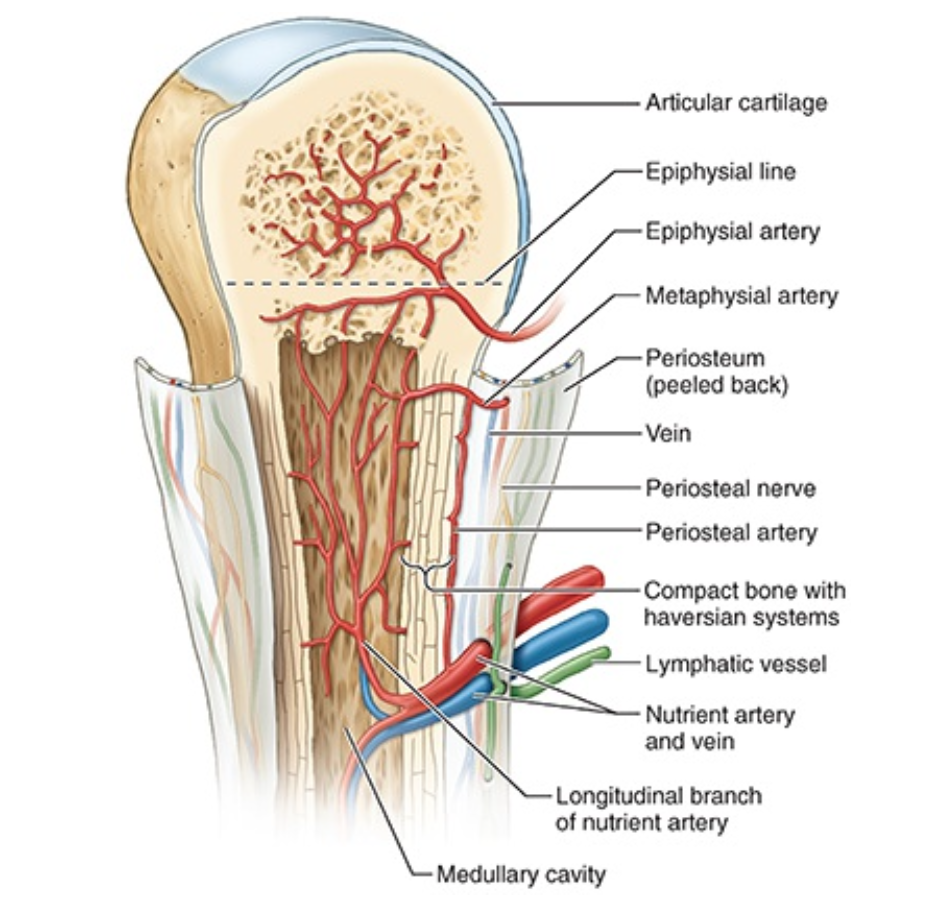
\includegraphics[width=0.5\linewidth]{Figures/blood_supply_of_bone.png}
    \caption{Vasculature and Innervation of a long bone. Taken from \cite[p.~120]{moore2023}}
    \label{fig:blood_supply_of_bone}
\end{figure}

\subsubsection*{Short Bone}
\textbf{Example:} Carpals, Tarsals\\
\textbf{Features:}
\begin{itemize}
    \item 6 surfaces (4 articular, 2 non-articular)
    \item Composed of spongy bone covered by thin shell of compact bone
    \item \textbf{Development:} Cartilaginous ossification, secondary ossification
    \item \textbf{Exceptions:} Talus, calcaneus and cuboid: primary ossification
\end{itemize}

\subsubsection*{Sesamoid Bone}
\textbf{Example:} Pisiform, Patella\\
\textbf{Features:}
\begin{itemize}
    \item Ossified from tendon of muscle
    \item Devoid of periosteum
    \item Devoid of Haversian system
\end{itemize}

\subsubsection*{Flat Bone}
\textbf{Example:} Frontal, Parietal\\
\textbf{Features:}
\begin{itemize}
    \item Two plates of compact bone with intervening spongy bone with bone marrow
    \item Form the boundary of some body cavity where protection of essential organs is needed
    \item \textbf{Development:} Membranous ossification
\end{itemize}
\textbf{Gross Structure:}
\begin{itemize}
    \item Periosteum
    \item Outer table
    \item Inner table
    \item Periosteum
\end{itemize}

\subsubsection*{Irregular Bone}
\textbf{Example:} Vertebrae\\
\textbf{Features:}
\begin{itemize}
    \item No specific geometrical shape
    \item Contains spongy bone and bone marrow
\end{itemize}

\subsubsection*{Pneumatic Bone}
\textbf{Example:} Frontal, Maxilla\\
\textbf{Features:}
\begin{itemize}
    \item Contains air cavity
    \item Lined by mucous membrane
    \item Close proximity to the nasal cavity
\end{itemize}
\textbf{Gross Structure:}
\begin{itemize}
    \item No periosteum
    \item Outer table (no Haversian system)
    \item Inner spongy bone
\end{itemize}

\subsubsection*{Accessory Bone}
\begin{itemize}
    \item Sometimes present in the body
\end{itemize}

\subsection{Classification According to Position}
The skeletal system may be divided into two functional parts\footnote{Moore mentions that the skeletal system, \textbf{not the bone} can be divided into two functional parts.\cite[~.p114]{moore2023}}.

\begin{itemize}
    \item The axial skeleton consists of the bones of the head (cranium or skull), neck (hyoid bone and cervical vertebrae), and trunk (ribs, sternum vertebrae, and sacrum).
    \item The appendicular skeleton consists of the bones of the limbs, including those forming the pectoral (shoulder) and pelvic girdles.
\end{itemize}

\subsection{Classification According to Gross Structure}
This is for the parts of bone, not the entire bone itself\footnote{A bone on and itself is not compact or spongy, parts of it are compact or spongy, for a flat bone, the outer and inner tables are compact while the middle is spongy, for a long bone, the covering is compact, which is thin at the ends, the shaft is compact almost all way through}.
\begin{itemize}
    \item Compact Bone
    \item Spongy Bone
\end{itemize}

\subsection{Classification According to Ossification}
The two process of bone formation is as follows\footnote{Both Gray and Moore mentions only two processes and that is according to formation.\cite[~.p96]{gray2020} \cite[~.p119]{moore2023}}
\begin{itemize}
    \item Membranous bone Formation (Intramembranous)
    \item Cartilaginous bone Formation (Endochondral)
    \item Membranocartilaginous bone\footnote{Some textbooks mention this}
\end{itemize}

\section{Regional Classification}
\subsection{Axial Skeleton}
\begin{itemize}
    \item Forms the vertical axis
    \item Consists of 80 bones
    \item \textbf{Example:}
    \begin{itemize}
        \item Skull
        \item Middle ear ossicles
        \item Hyoid Bone
        \item Vertebral Column
        \item Thoracic Cage
    \end{itemize}
\end{itemize}

\subsection{Appendicular Skeleton}
\begin{itemize}
    \item Consists of 126 bones
    \item Bones of the extremities including their anchors
    \item \textbf{Example:}
    \begin{itemize}
        \item Scapula
        \item Humerus
        \item Radius
        \item Ulna
        \item Carpals
        \item Metacarpals
        \item Phalanges
        \item Hip Bone
        \item Femur
        \item Patella
        \item Tibia
        \item Fibula
        \item Tarsals
        \item Metatarsals
        \item Phalanges
    \end{itemize}
\end{itemize}

\section{Microanatomy}

\subsection{Composition}

\subsubsection*{Cells (2\%)}
\begin{itemize}
    \item \textbf{Osteoprogenitor Cell}
    \begin{itemize}
        \item \textbf{Type:} Undifferentiated, pluripotent stem cell.
        \item \textbf{Location:} Inner layer of the periosteum and the endosteum.
        \item \textbf{Function:} Proliferates and differentiates into osteoblasts during growth and repair.
    \end{itemize}
    
    \item \textbf{Osteoblast} \textit{(Bone forming cell)}
    \begin{itemize}
        \item \textbf{Function:} Synthesizes osteoid (unmineralized matrix), including collagen fibers and ground substance. Facilitates mineral deposition.
        \item \textbf{Location:} Found in a layer on the surface of new bone matrix.
    \end{itemize}
    
    \item \textbf{Osteocyte}  \textit{(Bone maintaining cell)}
    \begin{itemize}
        \item \textbf{Origin:} A mature osteoblast that has become entrapped within the bone matrix it secreted.
        \item \textbf{Location:} Resides within a space called a \textit{lacuna}, found between the lamellae of an osteon.
        \item \textbf{Features:} 
        \begin{itemize}
            \item Most abundant cell type in mature bone.
            \item Possesses long cellular processes that connect to other osteocytes, forming a network.
            \item Function is to maintain the bone matrix and detect mechanical stress.
        \end{itemize}
    \end{itemize}
    
    \item \textbf{Osteoclast}  \textit{(Bone resorbing cell)}
    \begin{itemize}
        \item \textbf{Origin:} Large, multinucleated cell derived from the fusion of monocytes (macrophage lineage).
        \item \textbf{Location:} Found in depressions on the bone surface called \textit{Howship's lacunae}.
        \item \textbf{Function:} Resorbs bone tissue by secreting acids and enzymes, crucial for remodeling and calcium homeostasis.
    \end{itemize}
\end{itemize}

\subsubsection*{Extracellular Matrix (98\%)}
The matrix consists of an organic framework mineralized with inorganic salts.
\begin{itemize}
    \item \textbf{Organic Components (35\% of solids)}
    \begin{itemize}
        \item \textbf{Collagen Fibers (Type I):} Provide tensile strength and flexibility.
        \item \textbf{Ground Substance:} Comprises proteoglycans, glycosaminoglycans (GAGs) like hyaluronic acid and heparan sulfate, and other proteins.
    \end{itemize}
    
    \item \textbf{Inorganic Components (65\% of solids)}
    \begin{itemize}
        \item Primarily calcium phosphate in the form of \textbf{hydroxyapatite crystals} $\text{Ca}_{10}(\text{PO}_4)_6(\text{OH})_2$, which provides hardness and compressive strength.
        \item Also includes ions: bicarbonate, citrate, magnesium, potassium, and sodium.
    \end{itemize}
\end{itemize}

\subsection{Microscopic Organization}

\subsubsection*{Compact Bone}
\begin{itemize}
    \item The dense outer layer of bone. Its functional unit is the \textbf{Osteon} or \textbf{Haversian System}.
    \item \textbf{Components of an Osteon:}
    \begin{itemize}
        \item \textbf{Haversian Canal:} Central canal containing blood vessels, nerves, and connective tissue.
        \item \textbf{Concentric Lamellae:} Cylindrical layers of calcified matrix surrounding the central canal.
        \item \textbf{Lacunae:} Small cavities between lamellae that house osteocytes.
        \item \textbf{Canaliculi:} Tiny canals radiating from lacunae, connecting osteocytes and allowing nutrient/waste exchange.
        \item \textbf{Interstitial Lamellae:} Irregularly shaped fragments of old osteons filling the spaces between them.
    \end{itemize}
\end{itemize}

\subsubsection*{Spongy (Cancellous) Bone}
\begin{itemize}
    \item A network of bony struts and plates found inside bones, deep to the compact bone.
    \item \textbf{Composition:}
    \begin{itemize}
        \item \textbf{Trabeculae:} Interconnecting rods or plates of bone that are lined by a single layer of osteogenic cells (endosteum).
        \item \textbf{Lamellae:} The trabeculae are composed of a few irregular lamellae, not full osteons.
        \item \textbf{Marrow:} The spaces between trabeculae are filled with bone marrow (hematopoietic or fatty).
    \end{itemize}
\end{itemize}

\subsection{Covering Structures}

\subsubsection*{Periosteum}
A double-layered membrane covering the external surface of bones (except at joint surfaces).
\begin{itemize}
    \item \textbf{Outer Fibrous Layer:} Dense, irregular connective tissue (fibroblasts, collagen bundles).
    \item \textbf{Inner Cellular (Cambium) Layer:} Osteogenic; contains osteoprogenitor cells and osteoblasts.
\end{itemize}

\subsubsection*{Endosteum}
A single layer of osteoprogenitor cells and osteoblasts that lines all internal surfaces of bone, including the medullary cavity and the trabeculae of spongy bone.

\section{Development}
\subsection{Ossification (Osteogenesis)}
\begin{itemize}
    \item \textbf{Definition:} The process of bone formation.
    \item \textbf{Types:}
    \begin{itemize}
        \item Intramembranous Ossification
        \item Intracartilaginous (Endochondral) Ossification
    \end{itemize}
\end{itemize}

\subsubsection*{Intramembranous Ossification}
\begin{itemize}
    \item \textbf{Definition:} Bone forms directly within mesenchymal connective tissue.
    \item \textbf{Example:} Flat bones of the skull, clavicle.
    \item \textbf{Stages:}
    \begin{itemize}
        \item Mesenchymal condensation and appearance of centers of ossification.
        \item Formation of osteoid matrix and its calcification.
        \item Formation of spongy bone (trabeculae).
        \item Formation of compact bone and periosteum.
    \end{itemize}
\end{itemize}

\subsubsection*{Intracartilaginous (Endochondral) Ossification}
\begin{itemize}
    \item \textbf{Definition:} Bone forms by replacing a hyaline cartilage model.
    \item \textbf{Example:} Long bones, vertebrae.
    \item \textbf{Stages:}
    \begin{itemize}
        \item Chondrification: Formation of a hyaline cartilage model.
        \item Appearance of primary ossification center in the diaphysis.
        \item Formation of a periosteal bone collar.
        \item Invasion of periosteal buds, forming the medullary cavity.
        \item Appearance of secondary ossification centers in the epiphyses (after birth).
        \item Formation of epiphyseal growth plates.
    \end{itemize}
\end{itemize}

\subsection{Structure of a Growing Long Bone}
\begin{itemize}
    \item \textbf{Diaphysis:} The shaft, ossified from the primary center.
    \item \textbf{Metaphysis:} The epiphyseal end of the diaphysis.
    \item \textbf{Epiphysis:} The end part, ossified from a secondary center.
    \begin{itemize}
        \item \textbf{Types:}
        \begin{itemize}
            \item \textbf{Pressure Epiphysis:} Present at articular ends, involved in weight transmission (e.g., head of humerus).
            \item \textbf{Traction Epiphysis:} Non-articular, produced by muscle pull (e.g., trochanters of femur).
            \item \textbf{Atavistic Epiphysis:} Phylogenetically an independent bone (e.g., coracoid process).
            \item \textbf{Aberrant Epiphysis:} Not always present (e.g., epiphysis at head of 1st metacarpal).
        \end{itemize}
    \end{itemize}
    \item \textbf{Epiphyseal (Growth) Plate:}
    \begin{itemize}
        \item Thin plate of hyaline cartilage between diaphysis and epiphysis.
        \item Responsible for longitudinal growth.
        \item \textbf{Zones:}
        \begin{itemize}
            \item Zone of reserve cartilage
            \item Zone of proliferation
            \item Zone of hypertrophy
            \item Zone of calcified cartilage
            \item Zone of ossification
        \end{itemize}
        \item Disappears when bone growth stops.
    \end{itemize}
\end{itemize}

\subsection{Ossification Centers}
\begin{itemize}
    \item \textbf{Definition:} Sites where ossification begins.
    \item \textbf{Primary Ossification Center:}
    \begin{itemize}
        \item Appears before birth (usually by 4th month intrauterine).
        \item Located in the diaphysis.
        \item Usually single.
        \item \textbf{Exception:} Clavicle has two primary centers.
    \end{itemize}
    \item \textbf{Secondary Ossification Center:}
    \begin{itemize}
        \item Appears after birth (mostly) in the epiphyses.
        \item Can be single or multiple.
        \item \textbf{Exception:} Lower end of femur and upper end of tibia appear before birth.
    \end{itemize}
\end{itemize}

\subsection{Laws of Ossification}
\begin{itemize}
    \item Primary center appears before birth and is usually single.
    \item Secondary centers appear after birth and can be multiple.
    \item The nutrient foramen is directed away from the growing end.
    \begin{itemize}
        \item \textbf{Exception:} Fibula (directed towards the growing end).
    \end{itemize}
    \item The secondary center for a pressure epiphysis appears before that for a traction epiphysis.
    \item The secondary center that appears first, fuses last with the shaft.
    \begin{itemize}
        \item \textbf{Exception:} Lower end of fibula (appears first, fuses first).
    \end{itemize}
    \item Secondary centers fuse to form a single epiphysis (compound epiphysis), which then fuses with the diaphysis.
    \begin{itemize}
        \item \textbf{Exception:} Upper end of femur (three separate centers fuse independently in reverse order of appearance).
    \end{itemize}
    \item The epiphysis that appears first will unite last.
    \begin{itemize}
        \item \textbf{Exception:} Fibula (the growing end is the distal end).
    \end{itemize}
\end{itemize}

\printbibliography

\end{document}